\documentclass[aspectratio=169]{beamer}
\usepackage{hyperref}
\usepackage[T1]{fontenc}
\usepackage{NTU}
\usepackage[utf8]{inputenc}
%\usepackage{lmodern}


% other packages
\usepackage{latexsym,amsmath,xcolor,multicol,booktabs,calligra}
\usepackage{graphicx,pstricks,stackengine}

\usepackage[backend=bibtex,style=numeric]{biblatex}
\addbibresource{references.bib}

\author{Discente: Michel Tavares de Oliveira  \\ Orientador: Jean Carlos Teixeira de Araújo}
\title[Avaliação de desempenho, custo e eficiência
energética de linguagens de programação]{Avaliação de desempenho, custo e eficiência
energética de linguagens de programação}
%\subtitle{This is the Subtitle of Your Presentation}
\institute{Universidade Federal do Agreste de Pernambuco}
\date{Maio de 2024}


% defs
\def\cmd#1{\texttt{\color{red}\footnotesize $\backslash$#1}}
\def\env#1{\texttt{\color{blue}\footnotesize #1}}
\definecolor{deepblue}{rgb}{0,0,0.5}
\definecolor{deepred}{rgb}{0.6,0,0}
\definecolor{deepgreen}{rgb}{0,0.5,0}
\definecolor{halfgray}{gray}{0.55}

\begin{document}

\begin{frame}
    \titlepage
    \vspace{-10pt}
    \begin{figure}[htpb]
        \begin{center}
            
\includegraphics[width=0.13\linewidth]{images/ufapelogo.png}
        \end{center}
    \end{figure}
\end{frame}

\begin{frame}
    \tableofcontents[sectionstyle=show,subsectionstyle=show/shaded/hide,subsubsectionstyle=show/shaded/hide]
\end{frame}


\section{Motivacao}

\begin{frame}{Frame Title}
    \begin{itemize}
        \item A
        \item B
        \item C 
        \item D 
    \end{itemize}
\end{frame}


\section{Questões de pesquisa}

\begin{frame}{Questões de pesquisa}
    \begin{itemize}
        \item Questão de pesquisa 1. Qual linguagem de programação é mais eficiente energeticamente?
        \item Questão de pesquisa 2. A linguagem mais rápida, é mais eficiente energeticamente? 
        \item Questão de pesquisa 3. A linguagem que possui menor potência em Watts, foi a mais eficiente?
    \end{itemize}
\end{frame}



\section{Trabalhos ralacionados}

\begin{frame}{Trabalhos ralacionados}
    \begin{itemize}
        \item Energy efficiency across programming Languages: How Do Energy, Time, and
        Memory Relate?
        \item Towards a green ranking for programming languages
        \item Analyzing programming languages’s energy consumption: an empirical study
    \end{itemize}
\end{frame}



\section{Fundamentação teorica}

\subsection{Avaliação de desempenho de sistemas}
\begin{frame}{Avaliação de desempenho de sistemas}
    \begin{itemize}
        \item A
        \item B
        \item C 
        \item D 
    \end{itemize}
\end{frame}

\subsection{Green Software}
\begin{frame}{Green Software}
    \begin{itemize}
        \item A
        \item B
        \item C 
        \item D 
    \end{itemize}
\end{frame}

\subsection{Eficiência energética}
\begin{frame}{Eficiência energética}
    \begin{itemize}
        \item A
        \item B
        \item C 
        \item D 
    \end{itemize}
\end{frame}

\subsection{Métricas energéticas}

\begin{frame}{Joule}
    \begin{itemize}
        \item É a unidade de energia no Sistema Internacional de Unidades, utilizada para medir energia mecânica ou térmica
        \item Na energia mecânica 1 Joule equivale a energia nescessária aplicar força 1 Newton por 1 metro
        \item Na energia termica 1 Joule equivale a energia nescessária para aumentar a temperatuda da água a 1 grau
    \end{itemize}

\end{frame}

\begin{frame}{Watt}
    \begin{itemize}
        \item É a unidade de potencia no Sistema Internacional de Unidades, sendo a potencia media da quantidade de energia em um determinado tempo
        \item 1 Watt equivale a 1 Joule por segundo, logo, um dispositivo que consome 1 Watt está consummindo um Joule por segundo
    \end{itemize}
    \begin{equation}
        P = \frac{E}{t}
    \end{equation}
\end{frame}

\begin{frame}{Quilowatt}
    \begin{itemize}
        \item É uma unidade de potência referente a 1000 Watts
        \item Utilizada para medir portencia eletrica em aplicações residenciais e comerciais e industriais
    \end{itemize}
    \begin{equation}
        \text{Potência em quilowatts (kW)} = \frac{\text{Energia em kilojoules (kJ)}}{\text{Tempo em horas (h)}}
        \end{equation}
\end{frame}

\begin{frame}{Quilowatt-hora}
    \begin{itemize}
        \item Referente a energia produzida ou consumida no período de 1 hora
        \begin{equation}
            \text{Energia total (kWh)} = \text{Potência em Quilowatts (kW)} \times \text{Tempo total em horas (h)}
            \end{equation}
    \end{itemize}
\end{frame}




\section{Materiais,métodos e execução}

\subsection{Intel RAPL}
\begin{frame}{Intel RAPL}
    \begin{itemize}
        \item Otimizar o gerenciamento energético dos processadores Intel
        \item Monitoramento de alguns parametros como temperatura, potência e consumo energético
        \item Foi implementado a nível de hardware a partir da 6ª geração dos processadores Intel
        \item Segundo Khan at al 2018 \cite{khan2018IntelRapl}, a precisão do RAPL é bastante promisora e os valores reportados são precisos suficientemente para prever e modelar sistemas.
    \end{itemize}
\end{frame}

\begin{frame}{RAPL Power Domain}
    \begin{figure}
        \centering
        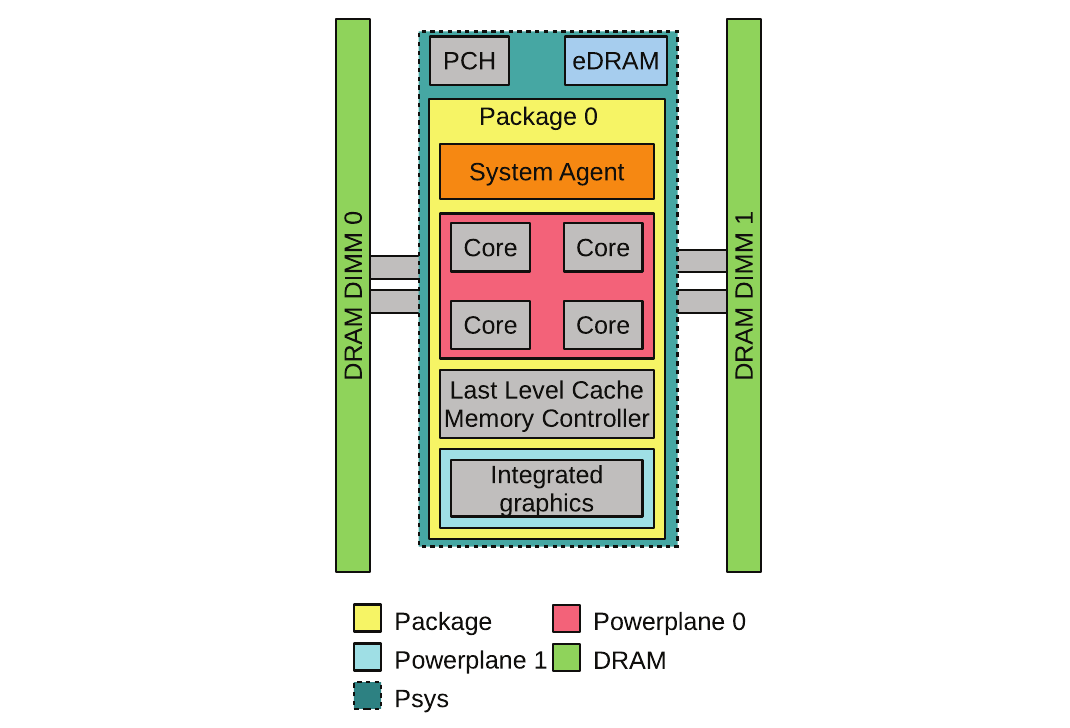
\includegraphics[width=0.61\linewidth]{images/powerDomainsRAPL.png}
        \caption{Intel RAPL Power Domains. Fonte: Khan at al 2018 \cite{khan2018IntelRapl}}
        \label{fig:powerDomains}
    \end{figure}
\end{frame}

\begin{frame}{Contadores de energia e limitações}
    \begin{itemize}
        \item Model-Specific Registers (MSRs) são registradores
        que fornecem acesso a diversas características e funcionalidades nos processadores x86
        \item MSR\_RAPL\_POWER\_UNIT de 32 bits sem sinal (0 a 4,294,967,295) 
        \item O registrador começa a contar a partir da inicialização do computador
        \item Quando este valor limite é atingido, o valor do registrador é reinicializado para 0 novamente.
        \item É de grande importância considerar a reinicialização
        dos registradores para não obter dados incorretos durante os experimentos
    \end{itemize}
\end{frame}

\subsection{Utilitários Linux}
\begin{frame}{Power Capping Framework}
    \begin{itemize}
        \item Ferramenta integrada ao Kernel Linux
        \item Permite expor informações de energia via \emph{sysfs} exportando informações sistemas de arquivos
        \item O framework cria de forma automática, uma árvore de diretórios com
        diversos objetos referente a interface de energia utilizada (The Linux Kernel Archives, 2024).
    \end{itemize}
\end{frame}

\begin{frame}{Árvore de Diretórios Power Capping Framework}
    \begin{figure}
        \centering
        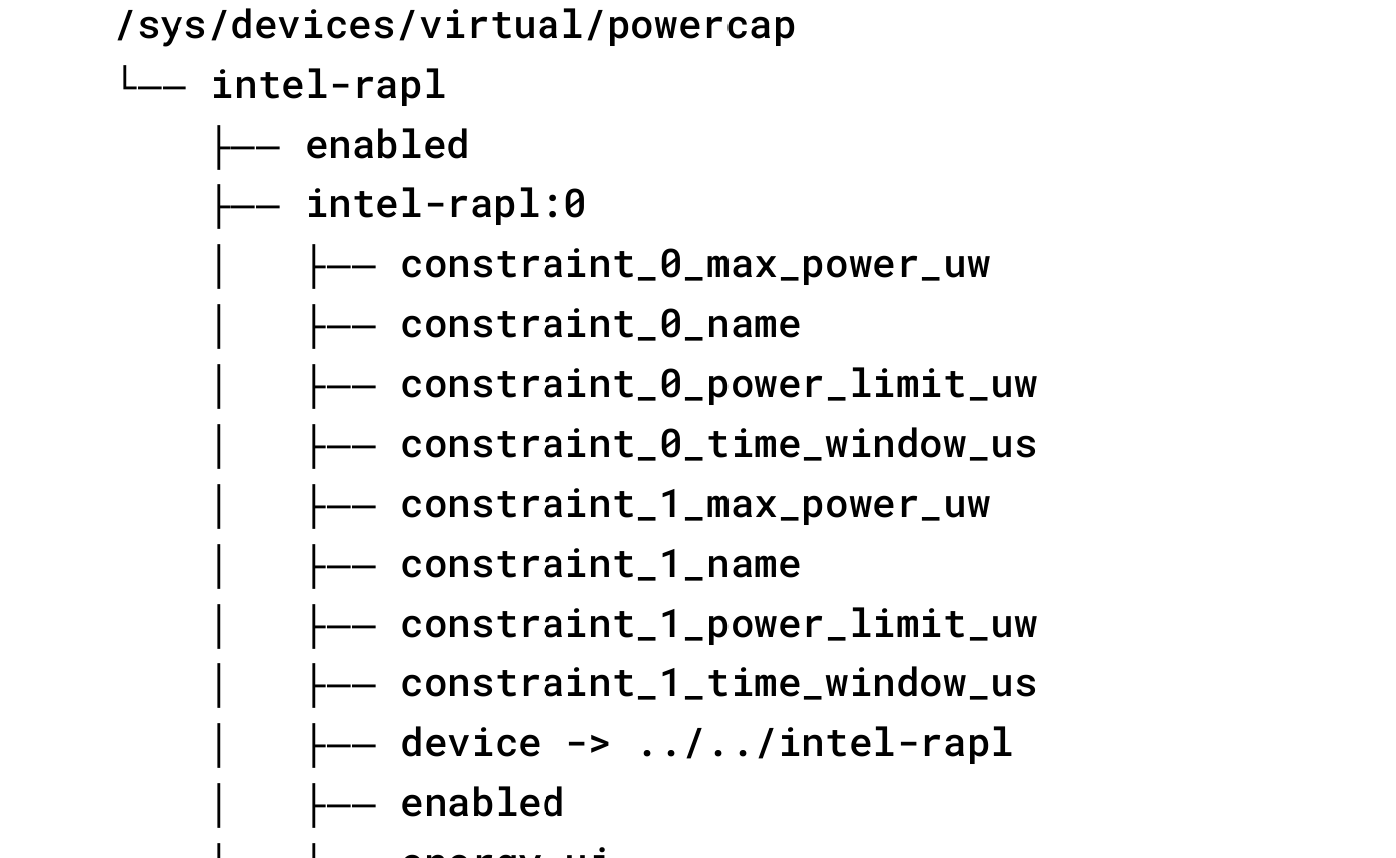
\includegraphics[width=0.65\linewidth]{images/powercap-tree.png}
        \caption{Árvore de Diretórios Power Capping Framework}
        \label{fig:powercap-tree}
    \end{figure}
\end{frame}

\begin{frame}{Shell}
    \begin{itemize}
        \item Interface entre o usuário e o sistema operacional
        \item O Shell é uma ferramenta essencial quando o foco é ter mais controle sobre o sistema operacional (RAYMOND, 2003)
        \item Funciona como um intermediário entre usuário e SO
        \item Essa interação pode ocorrer de forma iterativa e não iterativa
    \end{itemize}
\end{frame}

\begin{frame}{Shell Script}
    \begin{itemize}
        \item É uma linguagem de script voltada para automatização de tarefas em sistemas operacionais, sendo ela interpretada por um interpretador Shell
        \item Permite realizar diversas tarefas executando apenas um arquivo de script
        \item O interpretador analisa linha por linha e executa os comandos encontrados de forma sequencial
        \item Bastante útil ao executar diversos comandos, assim como a possibilidade de realização de tarefas repetitivas e automáticas
    \end{itemize}
\end{frame}

\begin{frame}{Bash}
    \begin{itemize}
        \item Bash é um shell desenvolvido por Brian Fox no Projeto GNU
        \item Atualmente é o Shell padrão de diversas distribuições Linux, como Ubuntu, Debian e Manjaro.
    \end{itemize}
\end{frame}

\begin{frame}{GNU Time}
    \begin{itemize}
        \item Utilizada para medir tempo e recursos consumidos por uma aplicação durante sua execução
        \item Utilização é bastante simples, com opções salvar a saída dos resultados em arquivo de texto
    \end{itemize}
    
    \begin{center}
        \texttt{/usr/bin/time ./meu\_programa > output.txt}
    \end{center}
\end{frame}

\subsection{The Computer Language Benchmark Game}
\begin{frame}{The Computer Language Benchmark Game}
    \begin{itemize}
        \item É um projeto de software livre que fornece um repositório com uma variedade de algorítimos simples que podem ser implementados em diversas linguagens de programação
        \item Um web site que centraliza todos os dados sobre códigos fontes, execução de teste e resultados
        \item O projeto fornece, além do código fonte, informações sobre compilação e execução dos algorítimos
    \end{itemize}
\end{frame}
\begin{frame}{CLBG Benchmarks}
	\centering
	
	\label{tbl:clbg_benchmarks}
	\begin{table}[h]

        \begin{tabular}{l|l}
        \textbf{Benchmarks} & \textbf{Descrição}   \\
        \hline
		fannkuch-redux      & Acesso indexado a minúsculas sequências inteiras            \\
		\hline
        n-body              & Dupla precisão para cálculo de N-body                       \\
		\hline
        spectral-norm       & Autovalor usando o método da potência                       \\
		\hline
        pidigits            & Streaming de aritmética de precisão arbitrária             \\
		\hline
        regex-redux         & Combina DNA e substitui por padrões mágicos                 \\
		\hline
        fasta               & Gerar e escrever sequências aleatórias de DNA               \\
		\hline
        k-nucleotide        & Atualiza hashtable e sequências de k-nucleotídeos           \\
		\hline
        reverse-complement  & Complemento reverso de sequências de DNA                     \\
		\hline
        binary-trees        & Aloca e desaloca muitas árvores binárias                    \\
		\hline
        mandelbrot          & Gera um conjunto de Mandelbrot em arquivo de bitmap portátil \\
    \end{tabular}
	\end{table}
\end{frame}

\subsection{Linguagens de Programação}
\begin{frame}{Linguagens de Programação}
    \begin{table}[h]
        \centering
        \fontsize{6}{7}\selectfont
        \begin{tabular}{l|l|l}
            \textbf{Linguagem} & \textbf{Versão} & \textbf{Compilador Open Source (Ubuntu 22.04)}\\
            \hline
            Ada & 10.5.1 & GNAT GPL Compiler \\
            \hline
            C & 11.4.0 & GCC \\
            \hline
            C\# & 7.0.115 & Mono \\
            \hline
            C++ & 11.4.0 & GCC \\
            \hline
            Chapel & 1.29.0 & Chapel Compiler \\
            \hline
            Dart & 3.2.6 & Dart SDK \\
            \hline
            Erlang &  26.2.2 & Erlang OTP \\
            \hline
            F\# & 7.0.115 & F\# Compiler \\
            \hline
            Fortran & 11.4.0 & GFortran \\
            \hline
            Go & 1.18.1 & Go Compiler \\
            \hline
            Haskell & 8.8.4 & GHC Haskell Compiler \\
            \hline
            Java & 19.0.2 & OpenJDK \\
            \hline
            Javascript & 18.19.0 & V8 \\
            \hline
            Julia & 1.9.3 & Julia Compiler \\
            \hline
            Lua & 5.3.0 & LuaJIT \\
            \hline
            Ocaml & 4.13.1 & OCaml Compiler \\
            \hline
            Perl & 5.34.1 & Perl Compiler \\
            \hline
            Php & 8.2.15 & PHP Compiler \\
            \hline
            Python & 3.10.12 & Python Interpreter \\
            \hline
            Racket & 8.2.0 & Racket Compiler \\
            \hline
            Ruby & 3.0.2 & Ruby Compiler \\
            \hline
            Rust & 1.75.0 & Rustc Compiler \\
            \hline
            Swift & 5.9.0 & Swift Compiler \\
        \end{tabular}
    \end{table}
\end{frame}


%\section{Execução}

\begin{frame}{Frame Title}
    \begin{itemize}
        \item A
        \item B
        \item C 
        \item D 
    \end{itemize}
\end{frame}


\section{Resultados}

\subsection{Análise das métricas por linguagem de programação}

\begin{frame}{Consumo em Joules por problema}
    \begin{figure}
        \centering
        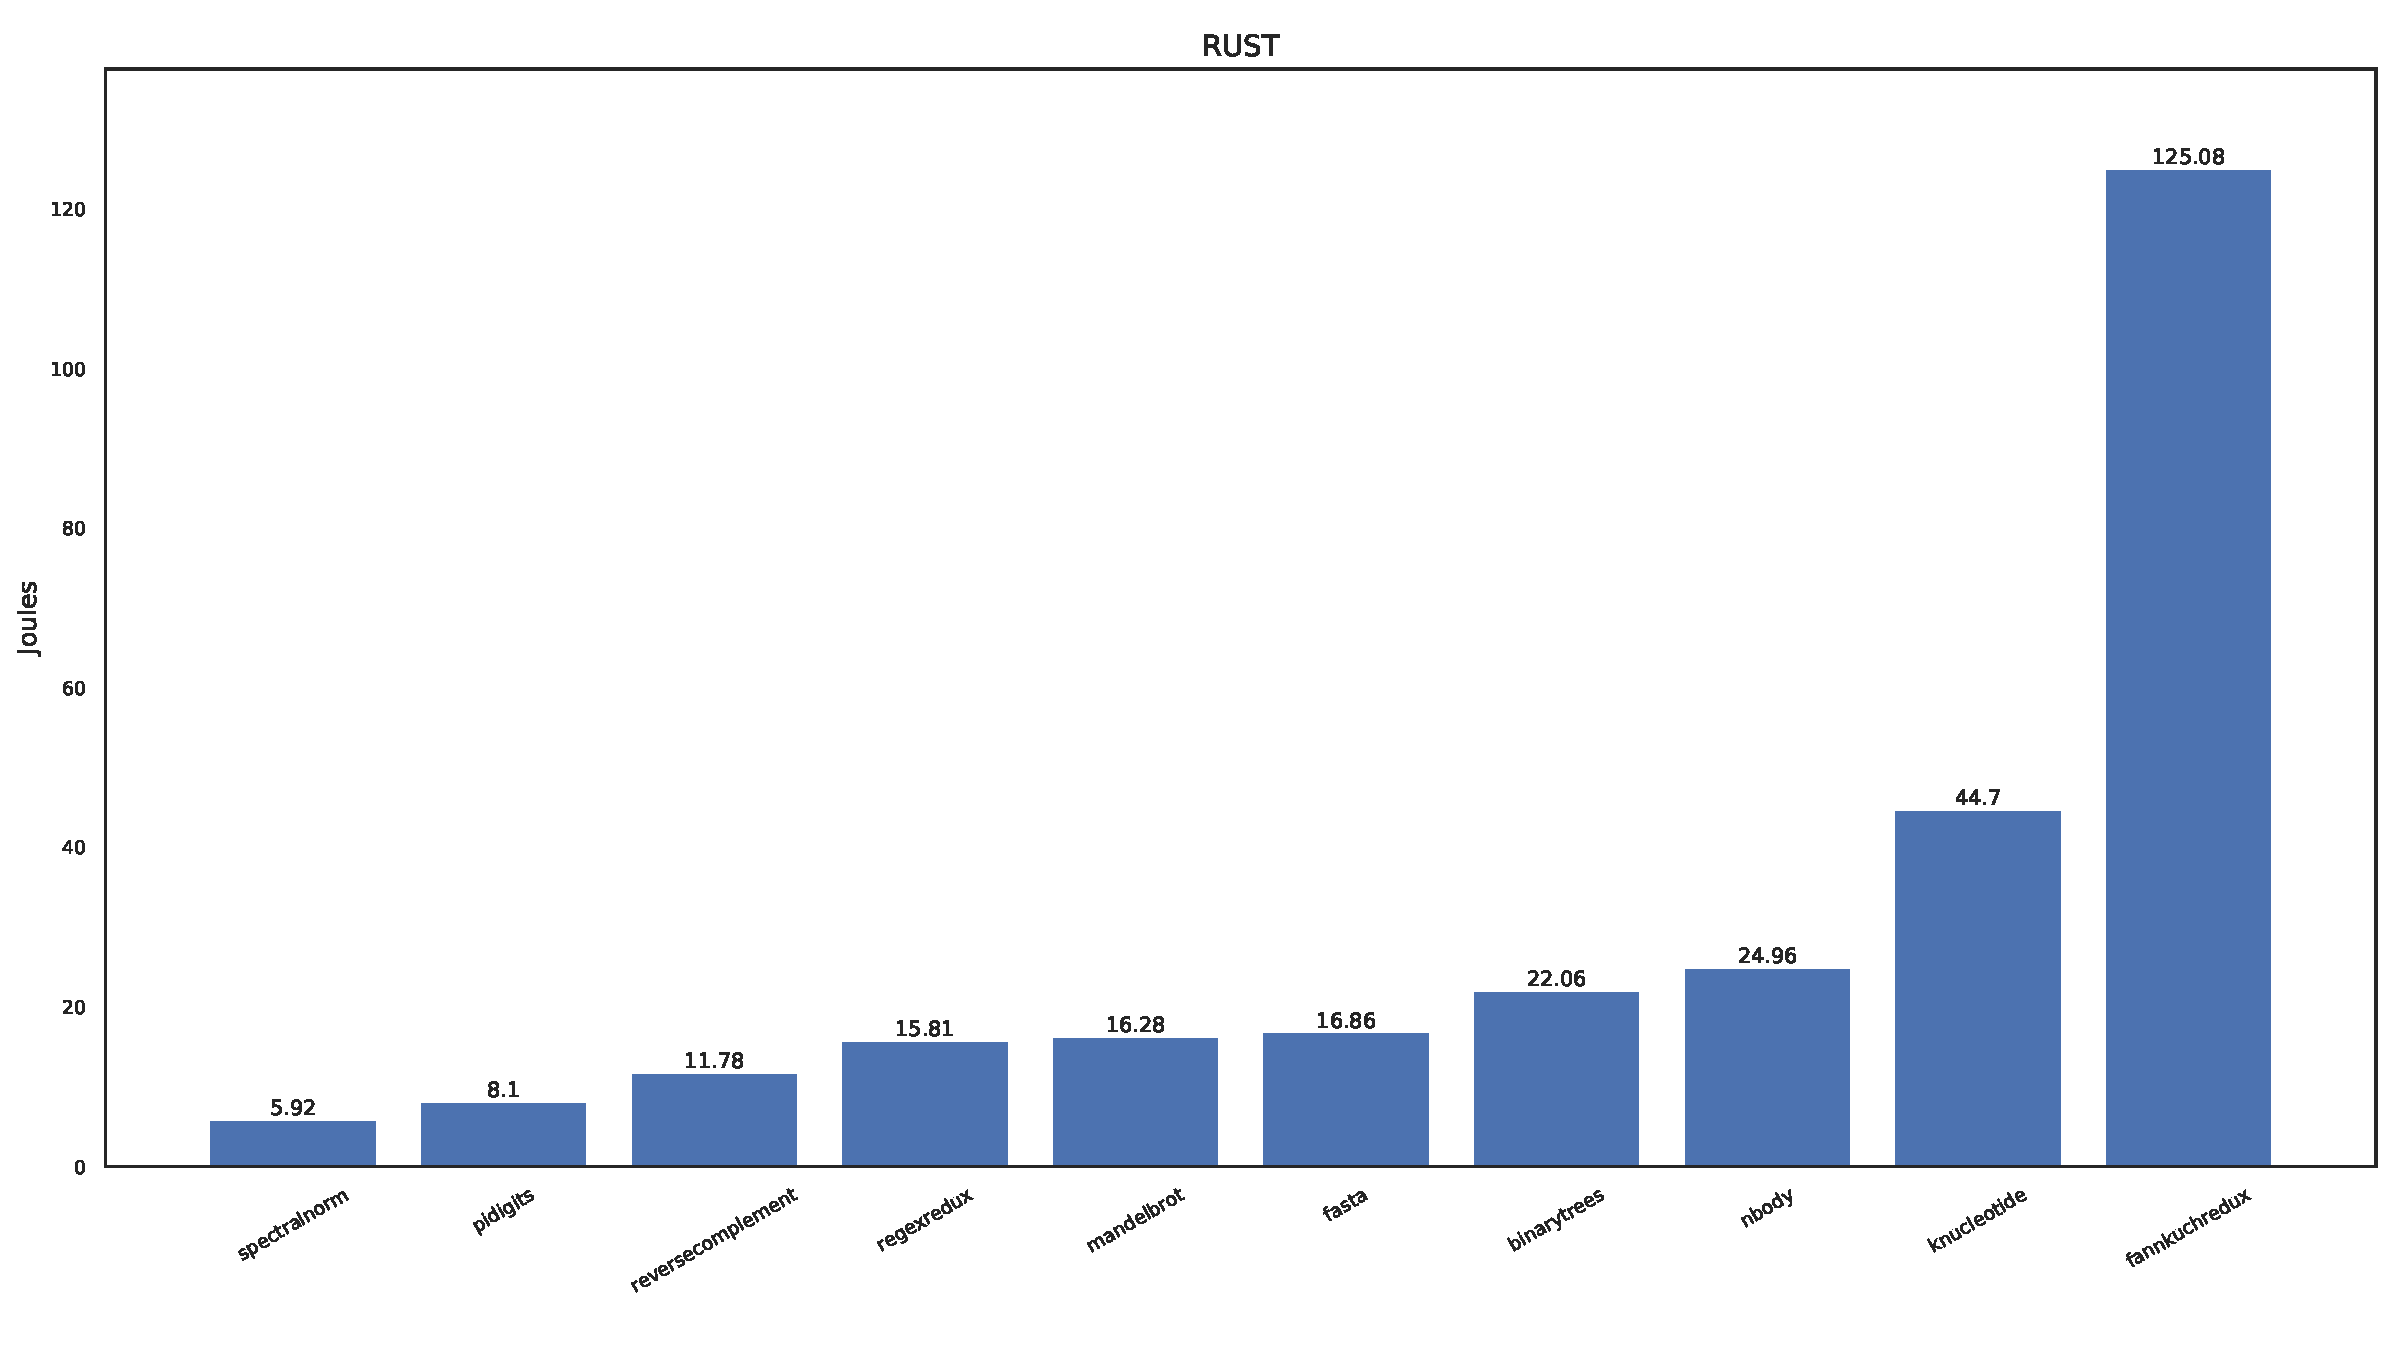
\includegraphics[width=0.85\linewidth]{images/rust-1.pdf}
        %\caption{Intel RAPL Power Domains. Fonte: Khan at al 2018 \cite{khan2018IntelRapl}}
        \label{fig:powerDomains2c3s4}
    \end{figure}
\end{frame}

\begin{frame}{Potência, memória, tempo e temperatura}
    \begin{figure}
        \centering
        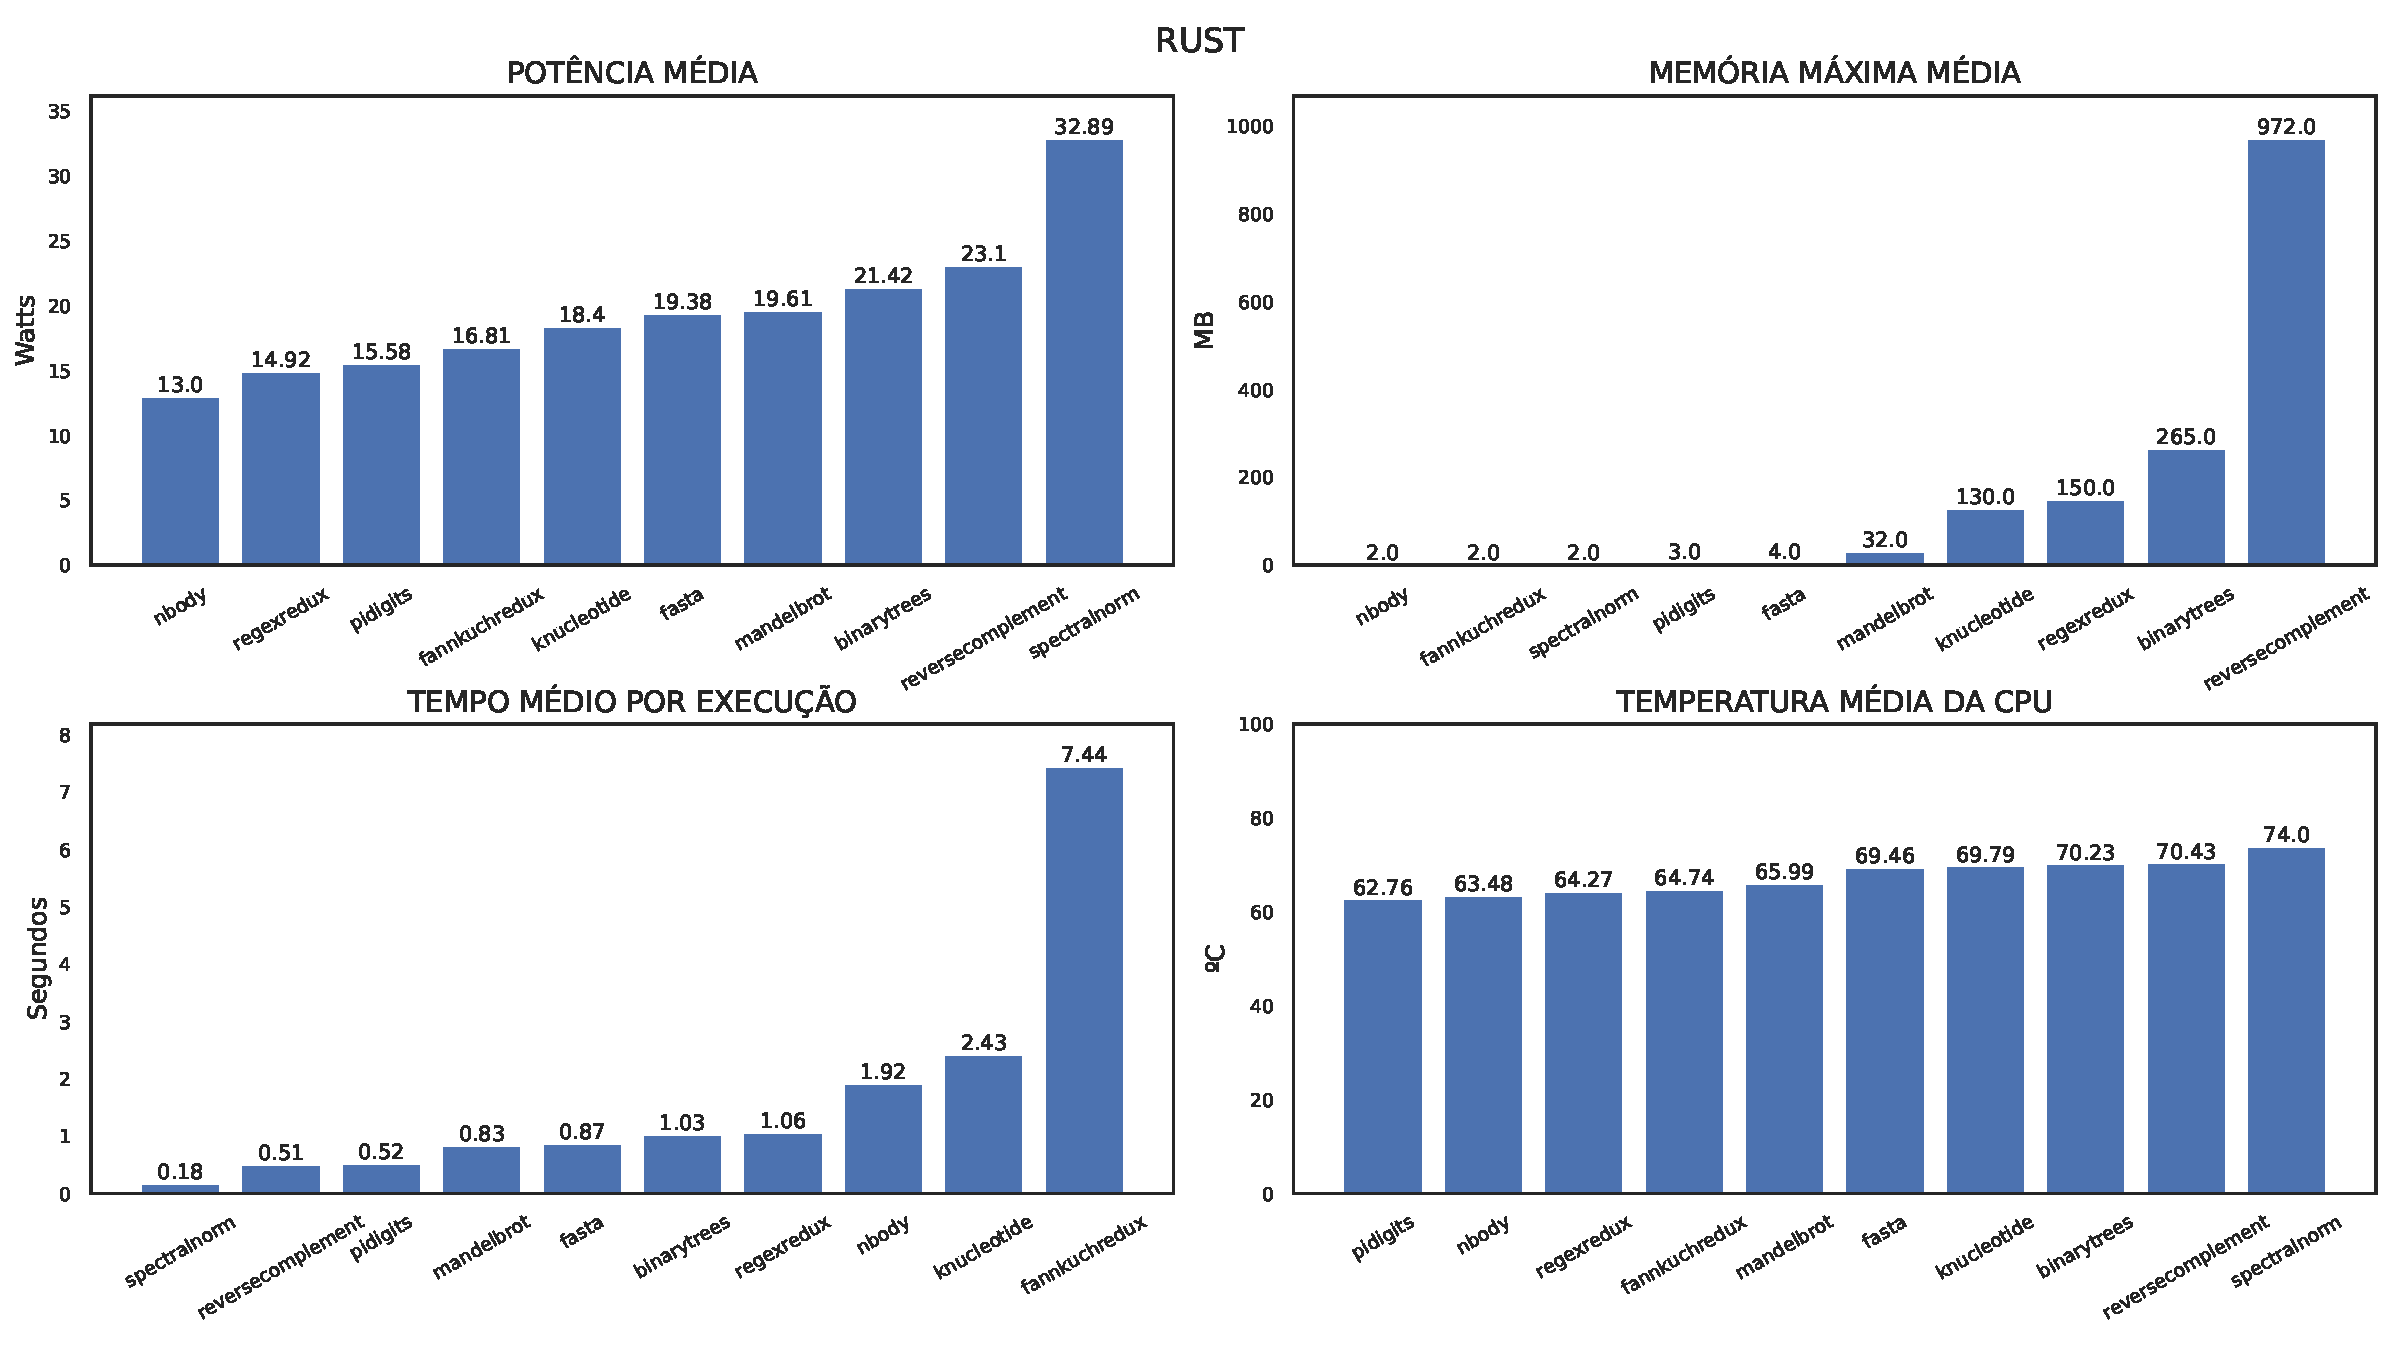
\includegraphics[width=0.85\linewidth]{images/rust-2.pdf}
        %\caption{Intel RAPL Power Domains. Fonte: Khan at al 2018 \cite{khan2018IntelRapl}}
        \label{fig:powerDomainsrusat2c3s4}
    \end{figure}
\end{frame}

\subsection{Eficiência energética}
\begin{frame}{Energia por execução}
    \begin{figure}
        \centering
        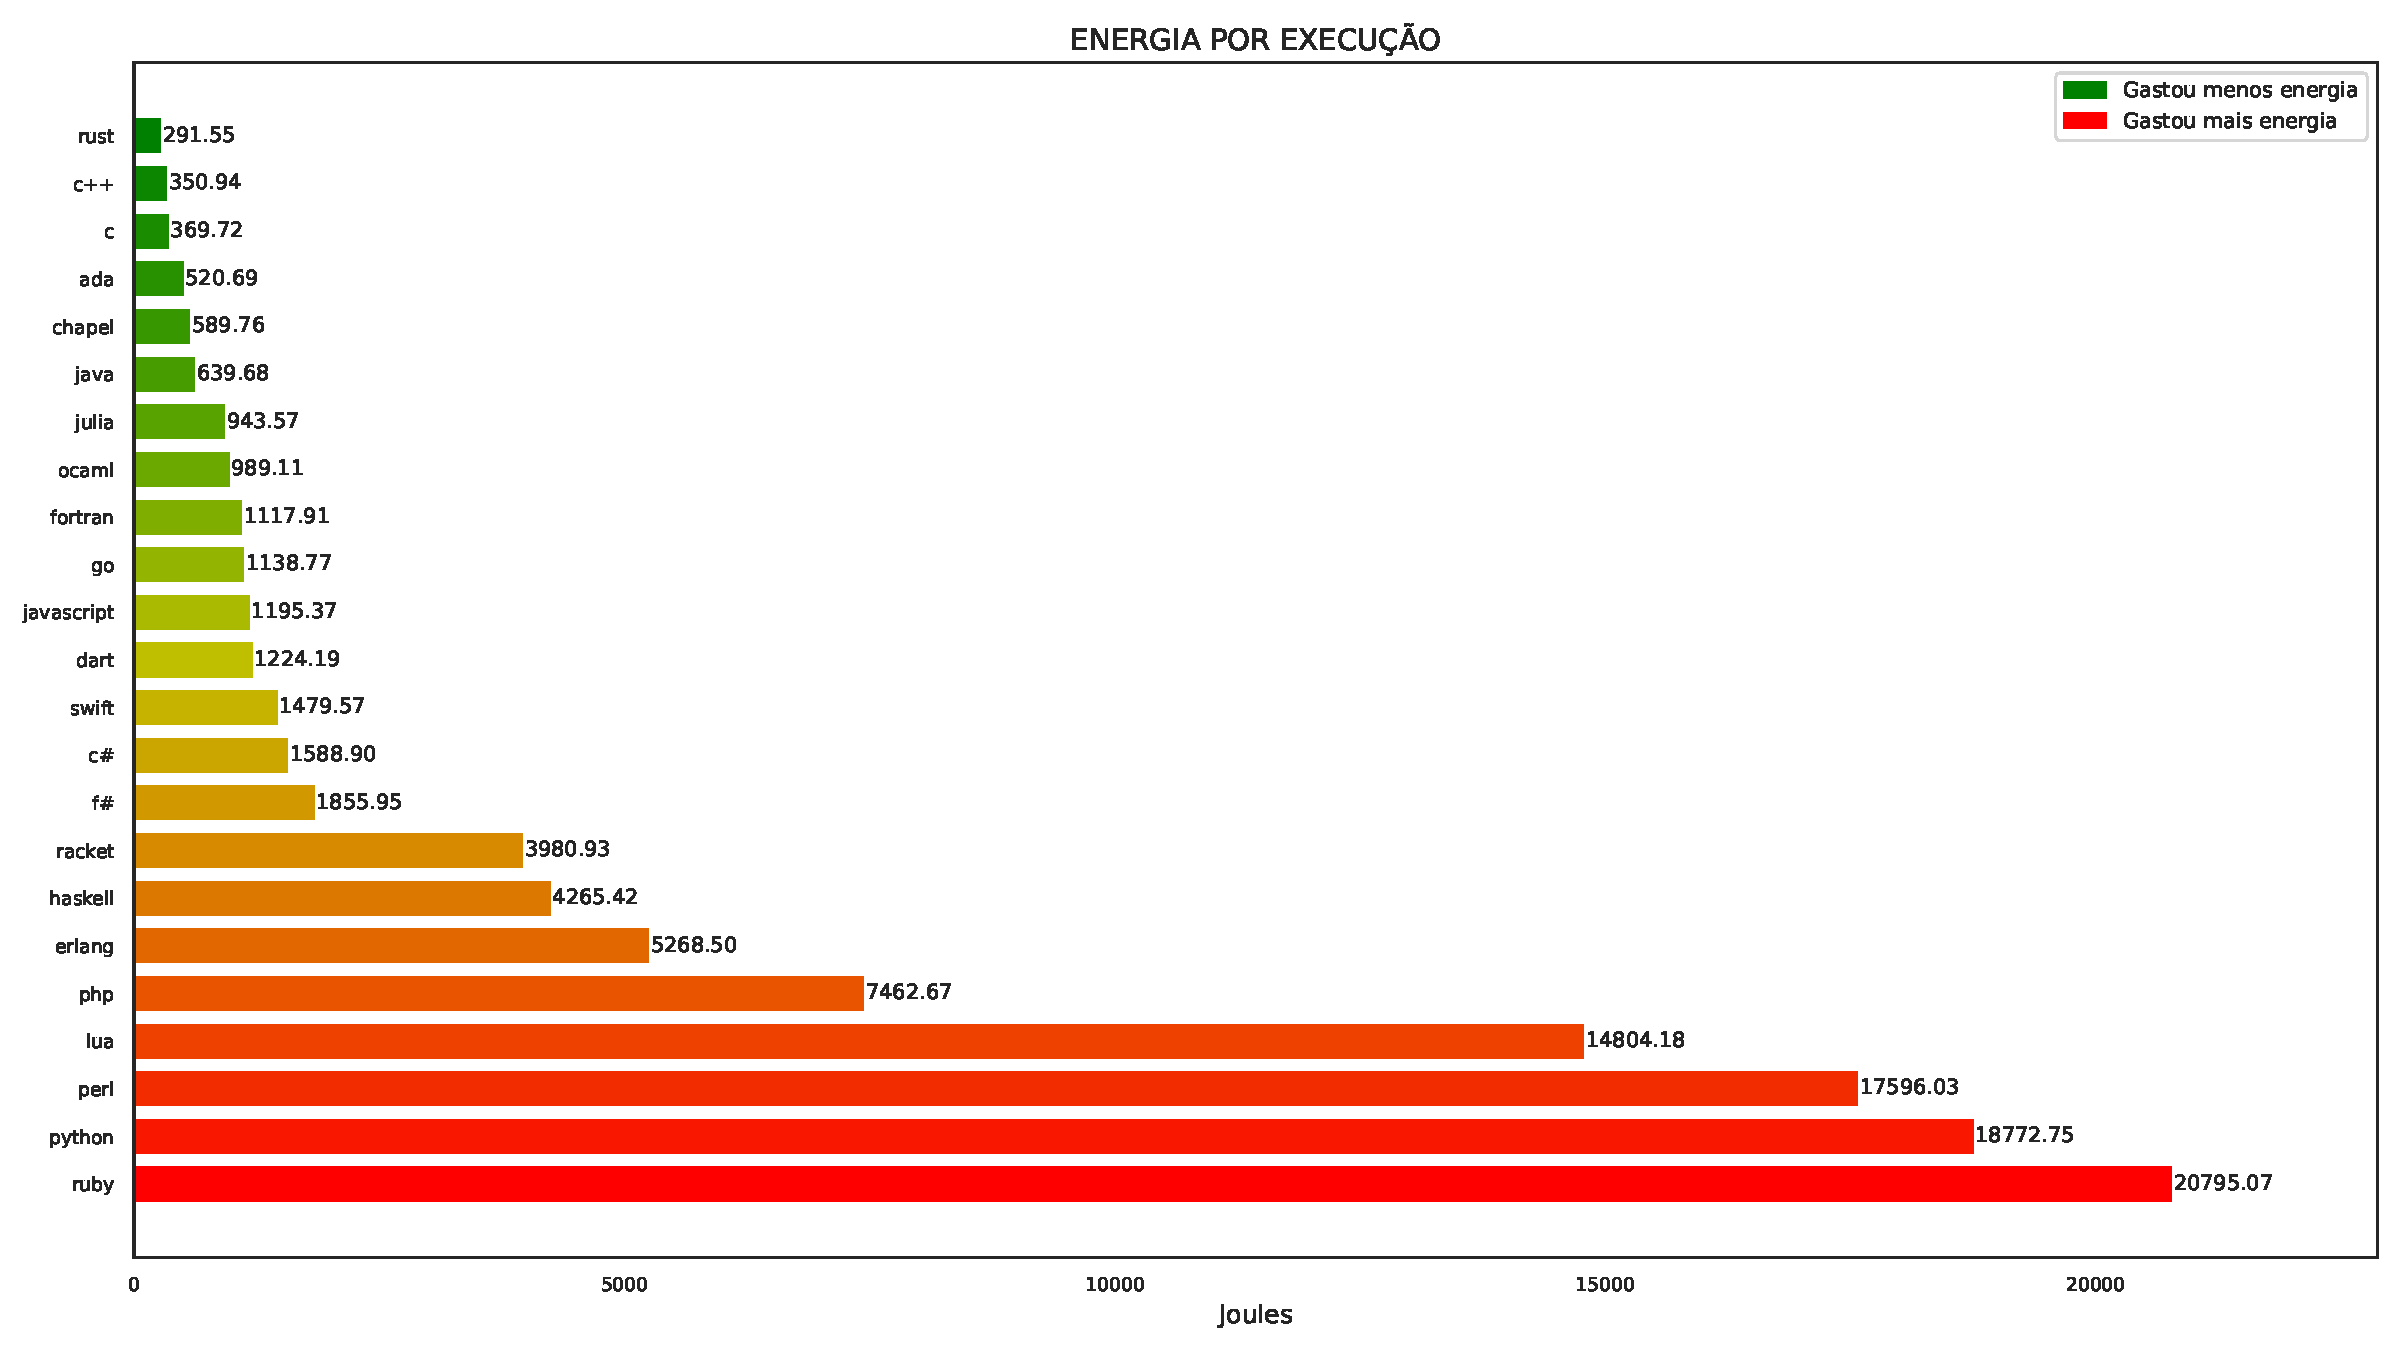
\includegraphics[width=0.85\linewidth]{images/energia_por_execucao.pdf}
        \caption{Intel RAPL Power Domains. Fonte: Khan at al 2018 \cite{khan2018IntelRapl}}
    \end{figure}
\end{frame}

\begin{frame}{Eficiência energética}
    \begin{figure}
        \centering
        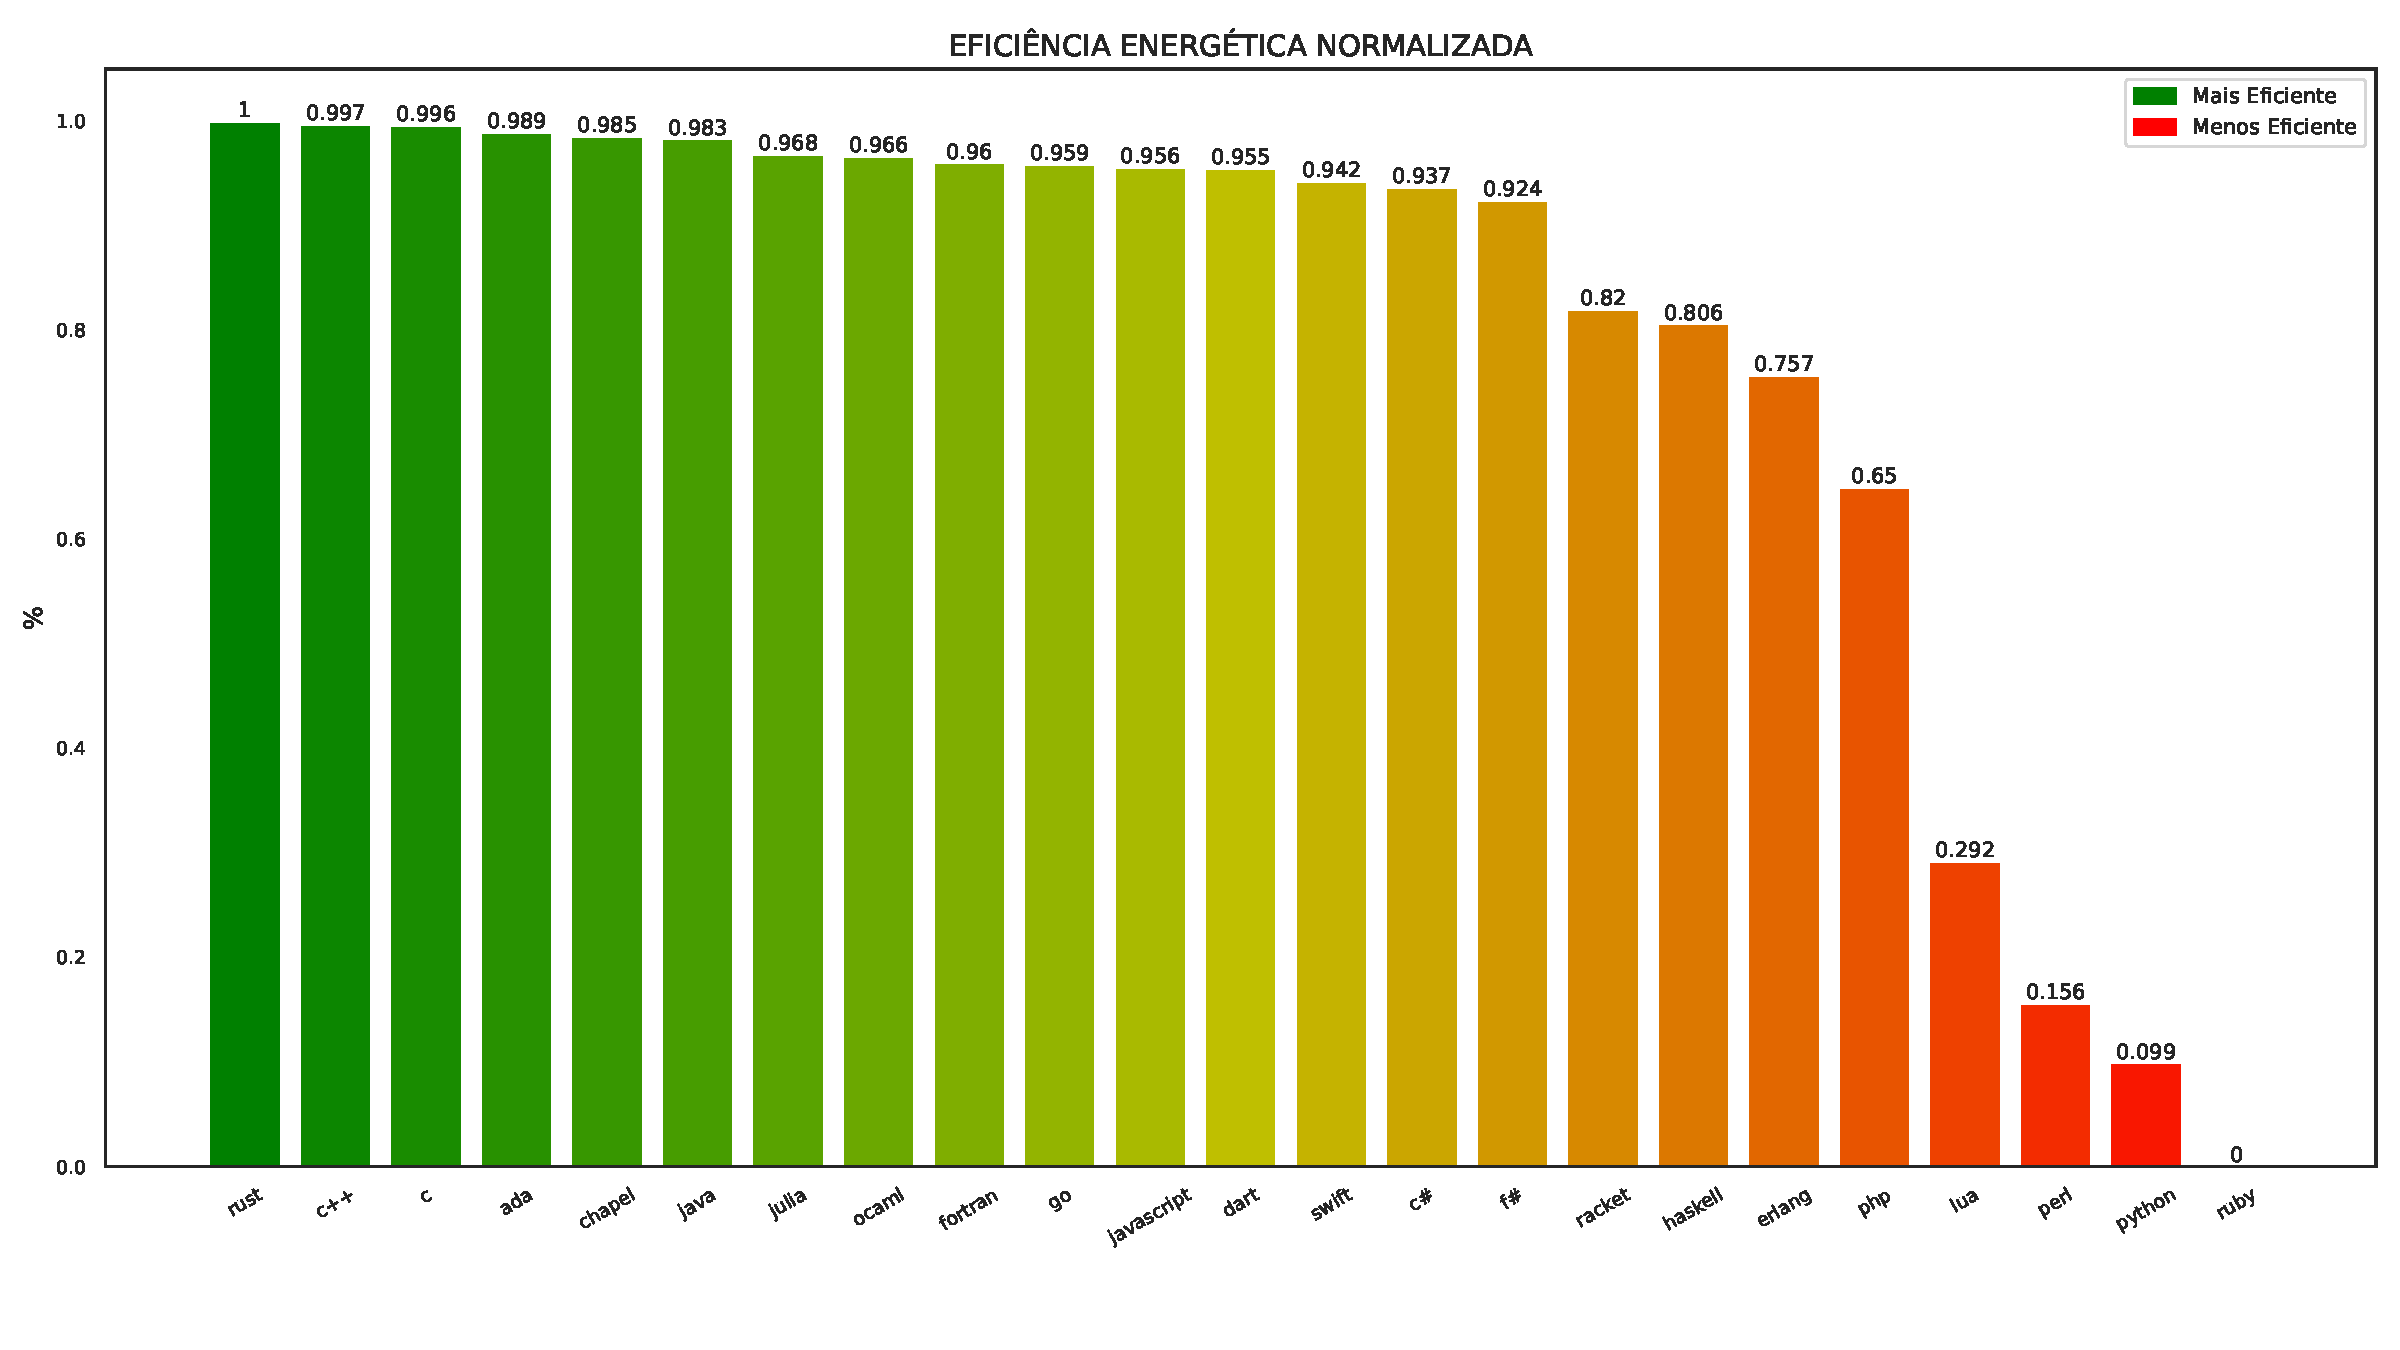
\includegraphics[width=0.85\linewidth]{images/eficiencia_energetica.pdf}
        %\caption{Intel RAPL Power Domains. Fonte: Khan at al 2018 \cite{khan2018IntelRapl}}
    \end{figure}
\end{frame}

\subsection{Análise do custo financeiro}
\begin{frame}{Análise do custo financeiro por 1000 execuções}
    \begin{itemize}
        \item A tarifa média considerada foi de 0.73 centavos por kWh
        \item Utilizamos o consumo total em Joules e convertemos para kWh
        \item Multiplicamos o consumo total em kWh por 1000 execuções
    \end{itemize}
 

    \begin{equation}
        \text{{Consumo em kWh}} = \frac{{\text{{Consumo em Joules}}}}{{3.600.000}}
    \end{equation}
\end{frame}

\begin{frame}{Linguagens de programação}
    \centering
    \begin{table}[!hp]
      %\caption{Linguagens de programação}
      %\label{tbl:custo}
      \centering
      %\rowcolors{2}{lightgray!30}{white}
      \fontsize{6}{7}\selectfont
      \begin{tabular}{l|l|l|l|l}
        \toprule
        \textbf{Linguagem} & \textbf{Joules} & \textbf{kWh} & \textbf{kWh por mil execuções} & \textbf{Custo por mil execuções (R\$)} \\
        \toprule
        Rust & 291,55 & 0,000081 & 0,081 & 0,05913 \\
        \hline
        C++ & 350,94 & 0,000098 & 0,098 & 0,07154 \\
        \hline
        C & 369,72 & 0,000103 & 0,103 & 0,07519 \\
        \hline
        Ada & 520,69 & 0,000145 & 0,145 & 0,10585 \\
        \hline
        Chapel & 589,76 & 0,000164 & 0,164 & 0,11972 \\
        \hline
        Java & 639,68 & 0,000178 & 0,178 & 0,12994 \\
        \hline
        Julia &  943,57 & 0,000262 & 0,262 & 0,19126 \\
        \hline
        Ocaml & 989,11 & 0,000275 & 0,275 & 0,20075 \\
        \hline
        Fortran & 1117,91 & 0,000310 & 0,310 & 0,2263 \\
        \hline
        Go & 1138,77 & 0,000316 & 0,316 & 0,23068 \\
        \hline
        Javascript & 1195,37 & 0,000332 & 0,332 & 0,24236 \\
        \hline
        Dart & 1224,19 & 0,000340 & 0,340 & 0,2482 \\
        \hline
        Swift & 1479,57 & 0,000411 & 0,411 & 0,30003 \\
        \hline
        C\# & 1588,90 & 0,000441 & 0,441 & 0,32193 \\
        \hline
        F\# & 1855,95 & 0,000516 & 0,516 & 0,37668 \\
        \hline
        Racket & 3980,93 & 0,001106 & 1,106 & 0,80738 \\
        \hline
        Haskell & 4265,42 & 0,001184 & 1,184 & 0,86432 \\
        \hline
        Erlang & 5268,50 & 0,001463 & 1,463 & 1,06799 \\
        \hline
        PHP & 7462,67 & 0,002073 & 2,073 & 1,51329 \\
        \hline
        Lua & 14804,18 & 0,004112 & 4,112 & 3,00176 \\
        \hline
        Perl & 17596,03 & 0,004888 & 4,888 & 3,56824 \\
        \hline
        Python & 18772,75 & 0,005214 & 5,214 & 3,80622 \\
        \hline
        Ruby & 20795,07 & 0,005777 & 5,777 & 4,21721 \\
        \bottomrule
      \end{tabular}
    \end{table}
\end{frame}


\section{Conclusão}

\begin{frame}{Qual linguagem de programação é mais eficiente energeticamente?}
    \begin{itemize}
        \item Rust (291.55 Joules)
        \item C++ (350.94 Joules)
        \item C (369.72 Joules)
    \end{itemize}
\end{frame}

\begin{frame}{A linguagem mais rápida, é mais eficiente energeticamente?}
    \begin{itemize}
        \item Não;
        \item Julia aoresentou maior tempo de execução em relação a Go e Chapel, mas conseguiu apresentar melhor eficiência, mesmo sendo mais lenta.
    \end{itemize}
\end{frame}

\begin{frame}{A linguagem que apresentou menor potência em watts, foi a mais eficiente?}
    \begin{itemize}
        \item Não;
        \item Pontência menor resulta em um maior tempo de execução;
        \item Linguagens com maior potência necessitavam de um menor tempo de execução.
    \end{itemize}
\end{frame}






\begin{frame}[allowframebreaks]
    \printbibliography
\end{frame}

\begin{frame}
    \begin{center}
        {\Huge EOF}
    \end{center}
\end{frame}

\end{document}
